\chapter{Schichttypen}\label{ch:schichten}

Eine Struktur ist ein Stapel von Schichten zwischen Substrat und Superstrat. Jede Schicht hat einen Typ, der
festlegt, wie ihr Querschnitt aussieht. Dieses Kapitel beschreibt jeden Typ mit allen Schlüsseln, einer Skizze und
einem Beispiel.

\begin{hinweis}[Gemeinsame Regeln]
\begin{itemize}[nosep]
  \item Längen in \textmu m; $x$-Koordinaten in $[0,d_x)$, $z$-Koordinaten in $[0,d_z)$.
  \item Materialnamen müssen in \key{materials} stehen.
  \item Fast alle Typen haben den optionalen Schlüssel \key{factorization} (Standard \val{"auto"},
        Kapitel~\ref{ch:loeser}).
  \item Die Dicke einer $y$-invarianten Schicht heißt \key{thickness\_um}, die einer Profilschicht \key{depth\_um}
        (Höhe des Profils von seinem tiefsten zum höchsten Punkt).
\end{itemize}
\end{hinweis}

%-------------------------------------------------------------------------------------------
\section{\texttt{homogeneous} -- homogene Schicht}
\index{Schichttyp!homogeneous@\texttt{homogeneous}}%
\begin{lstlisting}[language=json]
{ "type": "homogeneous", "thickness_um": 0.05, "material": "sio2" }
\end{lstlisting}
\begin{center}
\small
\begin{tabular}{lll}
\toprule
Schlüssel & Pflicht & Bedeutung \\
\midrule
\key{thickness\_um} & ja & Dicke \\
\key{material} & ja & Materialname (isotrop oder anisotrop) \\
\bottomrule
\end{tabular}
\end{center}
Typische Anwendungen: Deckschichten, Haftschichten, Antireflexschichten, Dünnschichtstapel (Airy-Formeln werden
exakt reproduziert, Referenzfall V2). Homogene Schichten sind in jeder Dimension und mit jedem Löser erlaubt und
kosten fast nichts.

%-------------------------------------------------------------------------------------------
\section{\texttt{lamellar1d} -- Lamellen}
\index{Schichttyp!lamellar1d@\texttt{lamellar1d}}\index{Lamellengitter}%
\begin{minipage}{0.55\linewidth}
\begin{lstlisting}[language=json]
{ "type": "lamellar1d",
  "thickness_um": 0.3,
  "breakpoints_um": [0.0, 0.2, 0.5, 1.0],
  "materials": ["au", "air", "sio2"] }
\end{lstlisting}
\end{minipage}\hfill
\begin{minipage}{0.4\linewidth}
\centering
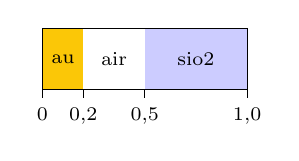
\begin{tikzpicture}[scale=2.6]
  \fill[yellow!60!orange] (0,0) rectangle (0.2,0.3);
  \fill[white] (0.2,0) rectangle (0.5,0.3);
  \fill[blue!20] (0.5,0) rectangle (1.0,0.3);
  \draw (0,0) rectangle (1,0.3);
  \foreach \x/\l in {0/0,0.2/0{,}2,0.5/0{,}5,1/1{,}0} \draw (\x,0) -- (\x,-0.04) node[below] {\scriptsize \l};
  \node at (0.1,0.15) {\scriptsize au}; \node at (0.35,0.15) {\scriptsize air}; \node at (0.75,0.15) {\scriptsize sio2};
\end{tikzpicture}
\end{minipage}

\begin{center}
\small
\begin{tabularx}{\linewidth}{llY}
\toprule
Schlüssel & Pflicht & Bedeutung \\
\midrule
\key{thickness\_um} & ja & Höhe der Lamellen \\
\key{breakpoints\_um} & ja & $K+1$ Stellen $0=x_0<x_1<\dots<x_K=d_x$ \\
\key{materials} & ja & $K$ Materialnamen, eines je Intervall $[x_{k},x_{k+1}]$ \\
\key{factorization} & nein & \val{auto} (= Li-Regeln für Lamellen), \val{laurent}, \val{li\_lamellar} \\
\bottomrule
\end{tabularx}
\end{center}
Lamellen dürfen beliebig viele Materialien haben, auch anisotrope. In 2D-Stapeln sind sie erlaubt und dann in $z$
invariant. Die Fourierkoeffizienten werden exakt berechnet; die Li-Regeln (Standard) machen TE und TM gleich schnell
konvergent. Zur Fehlervermeidung: Die Zahl der Stellen muss genau um eins größer sein als die Zahl der Materialien,
sonst meldet \FG{} \texttt{lamellar: breakpoints/materials}. Dass die erste Stelle 0 und die letzte gleich der
Periode ist, wird dagegen \emph{nicht} geprüft -- achten Sie selbst darauf, besonders wenn Sie die Periode ändern.

%-------------------------------------------------------------------------------------------
\section{\texttt{profile1d} -- Profil $y=g(x)$}\label{sec:profile1d}
\index{Schichttyp!profile1d@\texttt{profile1d}}\index{Sinusgitter}\index{Echelette}%
Eine Profilschicht trennt zwei Materialien durch eine Grenzfläche $y=g(x)$ mit $0\le g\le a$ (\key{depth\_um}).
Unterhalb liegt \key{below}, oberhalb \key{above}. Die Schicht ist so dick wie das Profil hoch ist.
\begin{center}
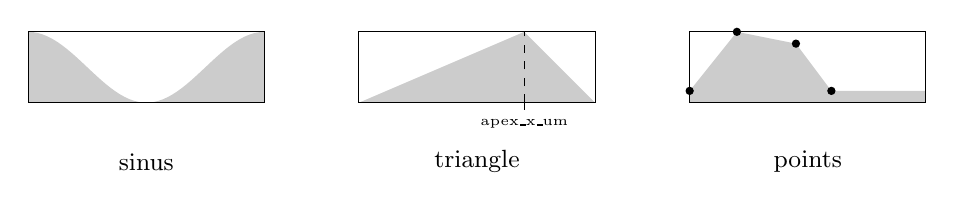
\begin{tikzpicture}[scale=3.0]
  \begin{scope}
    \fill[gray!40] (0,0) -- plot[domain=0:1,samples=50] (\x,{0.15*(1+cos(360*\x))}) -- (1,0) -- cycle;
    \draw (0,0) rectangle (1,0.3);
    \node at (0.5,-0.25) {\small \val{sinus}};
  \end{scope}
  \begin{scope}[xshift=1.4cm]
    \fill[gray!40] (0,0) -- (0.7,0.3) -- (1,0) -- cycle;
    \draw (0,0) rectangle (1,0.3);
    \draw[dashed] (0.7,0) -- (0.7,0.3);
    \draw (0.7,0) -- (0.7,-0.03) node[below] {\tiny \key{apex\_x\_um}};
    \node at (0.5,-0.25) {\small \val{triangle}};
  \end{scope}
  \begin{scope}[xshift=2.8cm]
    \fill[gray!40] (0,0) -- (0,0.05) -- (0.2,0.3) -- (0.45,0.25) -- (0.6,0.05) -- (1,0.05) -- (1,0) -- cycle;
    \draw (0,0) rectangle (1,0.3);
    \foreach \p in {(0,0.05),(0.2,0.3),(0.45,0.25),(0.6,0.05)} \fill \p circle (0.5pt);
    \node at (0.5,-0.25) {\small \val{points}};
  \end{scope}
\end{tikzpicture}
\end{center}
\begin{center}
\small
\begin{tabularx}{\linewidth}{lllY}
\toprule
Schlüssel & Pflicht & Standard & Bedeutung \\
\midrule
\key{depth\_um} & ja & & Profilhöhe $a$ \\
\key{below}, \key{above} & ja & & Material unter bzw.\ über der Grenzfläche \\
\key{shape} & nein & \val{sinus} & \val{sinus}, \val{triangle}, \val{points} \\
\key{x0\_um} & nein & 0 & \val{sinus}: Lage des Maximums \\
\key{apex\_x\_um} & bei \val{triangle} & & $x$-Lage der Spitze \\
\key{x\_um}, \key{y\_um} & bei \val{points} & & Stützstellen, $x$ aufsteigend in $[0,d_x)$ \\
\key{slices} & nein & 0 & RCWA-Scheiben dieser Schicht; 0 = \key{rcwa.slices} \\
\key{factorization} & nein & \val{auto} & siehe Tabelle~\ref{tab:faktorisierung} \\
\bottomrule
\end{tabularx}
\end{center}
\begin{description}
  \item[\val{sinus}] $g(x)=\tfrac a2\bigl(1+\cos K(x-x_0)\bigr)$ mit $K=2\pi/d_x$; das Maximum liegt bei $x_0$.
  \item[\val{triangle}] Dreieck (Echelette, Blazegitter): Von $(0,0)$ steigt die Flanke bis zur Spitze
        $(x_{\text{apex}},a)$ und fällt bis $(d_x,0)$ wieder ab. Der Blazewinkel ist
        $\arctan(a/x_{\text{apex}})$, der Gegenwinkel $\arctan\bigl(a/(d_x-x_{\text{apex}})\bigr)$.
  \item[\val{points}] Periodisches Polygon durch die Stützstellen $(x_i,y_i)$, stückweise linear verbunden und am
        Zellrand geschlossen. Die $y_i$ sollen in $[0,a]$ liegen.
\end{description}
\begin{lstlisting}[language=json]
{ "type": "profile1d", "shape": "triangle", "depth_um": 0.25, "apex_x_um": 0.7,
  "below": "au", "above": "air" }
\end{lstlisting}

\begin{hinweis}[Profile und Löser]
Der RK-Löser integriert Profile exakt (ohne Treppe); das ist der Hauptgrund, ihn zu verwenden. Mit RCWA wird das
Profil in \key{slices} Treppenstufen zerlegt; der Fehler fällt etwa mit $1/\text{slices}$. In 2D-Stapeln sind
isotrope \val{profile1d}-Schichten erlaubt und in $z$ invariant.
\end{hinweis}

%-------------------------------------------------------------------------------------------
\section{\texttt{polygon2d} -- Polygone und Rechtecke (2D)}\label{sec:polygon2d}
\index{Schichttyp!polygon2d@\texttt{polygon2d}}\index{Polygon}%
\begin{minipage}{0.58\linewidth}
\begin{lstlisting}[language=json]
{ "type": "polygon2d", "thickness_um": 0.2,
  "background": "ag",
  "inclusions": [
    { "material": "air",
      "rectangle_um": { "center": [0.45, 0.45],
                        "size": [0.25, 0.25] } },
    { "material": "sio2",
      "vertices_um": [[0.1,0.1],[0.2,0.1],[0.15,0.2]] }
  ],
  "normal_field": { "method": "tensor",
                    "grid": 512, "sigma": 3 },
  "factorization": "auto" }
\end{lstlisting}
\end{minipage}\hfill
\begin{minipage}{0.38\linewidth}
\centering
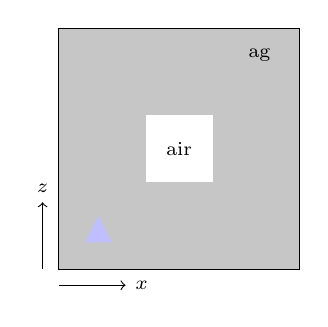
\begin{tikzpicture}[scale=3.4]
  \fill[gray!45] (0,0) rectangle (0.9,0.9);
  \fill[white] (0.325,0.325) rectangle (0.575,0.575);
  \fill[blue!25] (0.1,0.1) -- (0.2,0.1) -- (0.15,0.2) -- cycle;
  \draw (0,0) rectangle (0.9,0.9);
  \draw[->] (0,-0.06) -- (0.25,-0.06) node[right] {\scriptsize $x$};
  \draw[->] (-0.06,0) -- (-0.06,0.25) node[above] {\scriptsize $z$};
  \node at (0.45,0.45) {\scriptsize air};
  \node at (0.75,0.8) {\scriptsize ag};
\end{tikzpicture}

\small Querschnitt in der $(x,z)$-Zelle
\end{minipage}

Ein \val{polygon2d} ist ein in $y$ unveränderlicher Querschnitt: ein Hintergrundmaterial mit Einschlüssen. Jeder
Einschluss ist entweder ein Polygon (\key{vertices\_um}, Punkte $[x,z]$, mindestens drei, beliebiger Umlaufsinn)
oder ein achsenparalleles Rechteck (\key{rectangle\_um} mit \key{center} und \key{size}).
\begin{itemize}
  \item Polygone dürfen über den Zellrand hinausragen; ihre periodischen Bilder dürfen sich aber nicht überlappen.
  \item Einschlüsse dürfen sich nicht überlappen.
  \item Einschlüsse \emph{verschiedener} Materialien, die sich berühren, sind mit \val{FFF\_B} unzuverlässig
        (Abschnitt~\ref{ch:probleme}).
  \item Die Fourierkoeffizienten sind exakt (geschlossene Formeln für Polygone).
\end{itemize}
\paragraph{Normalenfeld.} Die FFF braucht in jedem Punkt der Zelle eine „Normalenrichtung“, die an den Rändern der
Einschlüsse senkrecht auf ihnen steht. \FG{} erzeugt sie auf einem Raster (Algorithmus NF):
\begin{center}
\small
\begin{tabularx}{\linewidth}{lllY}
\toprule
Schlüssel & Standard & & Bedeutung \\
\midrule
\key{method} & \val{tensor} & & \val{tensor}: geglättetes Projektorfeld $nn^T$ (vorzeichenfrei, robust); \val{vector}:
geglätteter Abstandsgradient (nur zwei Materialien) \\
\key{grid} & 512 & & Rasterpunkte je Periode (mindestens $8(2N+1)$ werden verwendet) \\
\key{sigma} & 3 & & Breite der Glättung in Rasterpunkten \\
\key{tau} & $10^{-3}$ & & nur \val{vector}: Rückfallschwelle \\
\bottomrule
\end{tabularx}
\end{center}
Das Normalenfeld beeinflusst nur die \emph{Konvergenzgeschwindigkeit}, nicht den Grenzwert. Die Standardwerte
sind fast immer richtig.

%-------------------------------------------------------------------------------------------
\section{\texttt{contour2d} -- gekrümmte Querschnitte (2D)}\label{sec:contour2d}
\index{Schichttyp!contour2d@\texttt{contour2d}}\index{NURBS}\index{Kreis, Ellipse}%
\val{contour2d} verallgemeinert \val{polygon2d} auf gekrümmte Ränder mit \emph{exakten} Fourierkoeffizienten:
Kreise und Ellipsen werden nicht durch Polygone angenähert.
\begin{lstlisting}[language=json]
{ "type": "contour2d", "thickness_um": 0.2, "background": "air",
  "regions": [
    { "material": "si", "circle":  { "center_um": [0.25, 0.25], "radius_um": 0.1 } },
    { "material": "si", "ellipse": { "center_um": [0.6, 0.6], "radii_um": [0.12, 0.06],
                                     "angle_deg": 30 } },
    { "material": "sio2", "polygon_um": [[0, 0], [0.1, 0], [0.1, 0.1]] },
    { "material": "si",
      "nurbs": { "degree": 2, "knots": [...], "points_um": [[x, z], ...], "weights": [...] },
      "holes": [ { "circle": { "center_um": [0.6, 0.2], "radius_um": 0.02 } } ] }
  ],
  "normal_field": { "grid": 512, "sigma": 3 },
  "factorization": "auto" }
\end{lstlisting}
\begin{center}
\small
\begin{tabularx}{\linewidth}{lY}
\toprule
Form & Schlüssel \\
\midrule
\key{circle} & \key{center\_um} $[x,z]$, \key{radius\_um} \\
\key{ellipse} & \key{center\_um}, \key{radii\_um} $[a,b]$, \key{angle\_deg} (Drehung, Standard 0) \\
\key{polygon\_um} & Liste von Punkten $[x,z]$ (identisch mit einem \val{polygon2d}-Polygon) \\
\key{nurbs} & \key{degree}, \key{knots} (geklemmt), \key{points\_um}, optional \key{weights}; geschlossen: erster
$=$ letzter Punkt \\
\key{holes} & Liste weiterer Formen, die aus der Region ausgeschnitten werden \\
\bottomrule
\end{tabularx}
\end{center}
Regionen müssen paarweise disjunkt sein, auch mit ihren periodischen Bildern; das wird geprüft. Faktorisierung:
\val{auto} (= \val{FFF\_sym} isotrop, \val{FFF\_B} anisotrop), \val{FFF\_iso}, \val{laurent}. Kreise und Ellipsen sind
intern exakte rationale Kurven; die Koeffizienten stimmen auf etwa $10^{-14}$. Der Referenzfall V15 zeigt, dass
Polygone mit $L$ Ecken mit einem Fehler $\propto L^{-2}$ gegen den exakten Kreis konvergieren -- ein guter Grund,
Kreise als \key{circle} statt als Vieleck anzugeben.

%-------------------------------------------------------------------------------------------
\section{\texttt{profile2d} -- Profil $y=g(x,z)$ (2D)}
\index{Schichttyp!profile2d@\texttt{profile2d}}%
\begin{lstlisting}[language=json]
{ "type": "profile2d", "shape": "egg_crate", "depth_um": 0.1,
  "below": "si", "above": "air", "x0_um": 0, "z0_um": 0,
  "slices": 0, "z_samples": 0, "factorization": "auto" }
\end{lstlisting}
\begin{description}
  \item[\val{egg\_crate}] $g=\tfrac a4\bigl(1+\cos K_x(x-x_0)\bigr)\bigl(1+\cos K_z(z-z_0)\bigr)$ -- „Eierkarton“.
  \item[\val{sinus\_x}] $g=\tfrac a2\bigl(1+\cos K_x(x-x_0)\bigr)$, invariant in $z$ (Test gegen 1D).
\end{description}
\key{slices} wie bei \val{profile1d}; \key{z\_samples} steuert die Abtastung in $z$ (0 = automatisch). Standard der
Faktorisierung ist \val{FFF\_rig} (isotrop) bzw.\ \val{FFF\_A} (anisotrop). Eigene Profilfunktionen $g(x,z)$ sind
über die C++-Schnittstelle möglich (Kapitel~\ref{ch:cpp}).

\begin{achtung}[Rechenaufwand]
2D-Profile sind die teuersten Strukturen: Jede der \key{slices} Scheiben braucht ein eigenes Eigenwertproblem der
Größe $4n_f$. Mit RK ist der Aufwand noch höher. Beginnen Sie mit kleinem $N$ (4--5) und 20 Scheiben.
\end{achtung}

%-------------------------------------------------------------------------------------------
\section{\texttt{cad} -- STEP-Körper}
\index{Schichttyp!cad@\texttt{cad}}%
Eine \val{cad}-Schicht liest Körper aus einer STEP-Datei und zerlegt sie beim Laden in Bänder aus homogenen,
\val{contour2d}- und $y$-variablen Schichten. Sie hat eigene Schlüssel und ein eigenes Kapitel
(Kapitel~\ref{ch:cad}).

%-------------------------------------------------------------------------------------------
\section{\texttt{rings} -- konzentrische Ringe (Zylinder)}
\index{Schichttyp!rings@\texttt{rings}}%
Nur in rotationssymmetrischen Rechnungen (Block \key{cylindrical}, Abschnitt~\ref{sec:zylinder}):
\begin{lstlisting}[language=json]
{ "type": "rings", "thickness_um": 0.3, "radii_um": [0.4], "materials": ["sin", "air"] }
\end{lstlisting}
$n$ Radien und $n+1$ Materialien von innen nach außen; das letzte Material gilt außerhalb des größten Radius bis ins
Unendliche. Das Beispiel ist eine Säule aus \texttt{sin} mit Radius 0,4\um.

%-------------------------------------------------------------------------------------------
\section{Schichten kombinieren}
Schichten verschiedener Typen dürfen beliebig gestapelt werden. Einige Beispiele:
\begin{itemize}
  \item \textbf{Gitter mit Deckschicht}: \val{lamellar1d}, darüber \val{homogeneous}.
  \item \textbf{Geätztes Profil in einem Film}: \val{homogeneous} (Restfilm), darüber \val{profile1d} mit
        \key{below} = Filmmaterial.
  \item \textbf{Säulen mit Kappe}: zwei \val{contour2d}-Schichten mit verschiedenen Radien.
  \item \textbf{Schräge Wände in 2D}: mehrere dünne \val{polygon2d}-Schichten mit schrittweise veränderter Größe
        (manuelle Treppe) oder besser eine \val{cad}-Schicht.
\end{itemize}
Achten Sie darauf, dass sich die Materialien an Schichtgrenzen physikalisch sinnvoll fortsetzen. \FG{} prüft das
nicht: Ein Steg aus Gold kann auf einem Steg aus Luft stehen.
